\chapter*{Conclusion}

\begin{figure}[h]
    \captionsetup{labelformat=empty}
    \hspace{\stretch{1}} 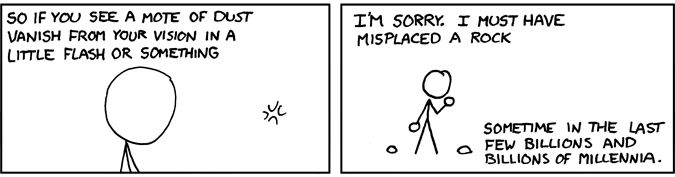
\includegraphics[width=0.75\textwidth]{xkcd/xkcd8.png}
    \caption*{\hspace{\stretch{1}}  Randall Munroe, \emph{A Bunch of Rocks} (part 8 of 9), \texttt{xkcd.com/505/} }
\end{figure}


In chapter~\ref{ch-1}, we made a contribution to quantum entanglement theory by introducing a new entanglement criterion, the Schrodinger-Robertson partial transpose inequality. We took advantage of the physicality of a partially transposed separable state to constrain the product of the variances of two operators to a minimal value. The violation of that constraint when measured on some state is the indisputable sign of entanglement in the state. We showed that not just any operator could be used in that inequality, and we gave a precise description of acceptable operators. We proved that there is always a pair of suitable operators that are able to detect the entanglement of any pure bipartite state of any dimension, giving a necessary and sufficient criterion for the detection of entanglement. We also proved that the criterion was necessary and sufficient in the case of pure three-qubit state. The Schrodinger-Robertson partial transpose inequality has a very wide range of application and we tested it on a few systems, multipartite mixed states, harmonic oscillators, multiphoton polarization states, continuous variable states or Schrodinger cat states with very encouraging results.

In chapter~\ref{chap-conc}, we introduced an $N$-qubit generalization of the concurrence, originally defined for two qubits. We started off with three qubits and we gave a series of conditions that we proved to be necessary and sufficient for the entanglement of pure states. We used these conditions to construct nine matrices that lead to the definition of the three-qubit concurrences for pure states. We showed that those concurrences were not unrelated to other established measures of entanglement, such as the three-tangle or another type of multipartite concurrence defined in the literature. Following in the footsteps of the original concurrence, we generalized the application of our concurrences to mixed sates and we showed that any linear combination of the nine original matrices could be used to define a concurrence applicable on mixed states. Any observed non-zero concurrence in a state immediately indicates the presence of entanglement in the system. We showed that in the case of symmetric states, the number of concurrences could be reduced to three, with which a non-zero value  directly indicates the presence of genuine tripartite entanglement. We pushed the generalization to $N$-qubit states by determining all the necessary and sufficient conditions to entanglement of a pure state. Those conditions allowed us to define the concurrences for pure and mixed states of $N$-qubits. We concluded with an example application on a family of mixed states into which any $N$-qubit state can be depolarized and saw that the entanglement of those state could always be detected with our concurrences.

In chapter~\ref{ch-3}, we started to get interested in ways to produce entanglement in physical systems such as cold atoms. We investigated the dipole blockade effect observed in such systems and modelized it with an interaction term in the Hamiltonian and master equation of the system. We showed that if the doubly excited state was shifted out of resonance far enough, the system would evolve from the ground state into a mixture of ground state and maximally entangled state. We measured the intensity of the blockade as well as the concurrence in different situations and we concluded that indeed the amplitude of the blockade in the system was a good marker for the amount of entanglement shared in the atoms. We also saw that the blockade could be lifted by considering a strong enough laser excitation. This observation lead us to investigate the steady state of the system towards which all  systems tend to. We were able to find the analytical expression of the steady state, which allowed us to give the expression for the amplitude of the blockade. Furthermore, we were able to give an analytical expression of the concurrence in the state. This expression can be used to calculate the laser strength that will maximize the amount of entanglement in the system for a given interaction strength. We concluded the chapter by giving another way to probe the blockade effect in the system, the photon-photon correlation. We showed a connection between values of the photon-photon correlation and the blockade, which provides a new way to measure the effect in an atomic system in the case where the spontaneous emission dominates over other dissipation effects.

In chapter~\ref{ch-4}, we extended our model to three-atom systems. We showed that it was enough to consider the sum of the pairwise atomic interactions to find the global interactive terms in the Hamiltonian. We studied the system in a mixed symmetry basis that helped us along the way to interpret several results. After a few considerations on  general configurations of the system, we studied different cases: no interaction between the atoms, interaction between only two, same interaction between all atoms and aligned atoms with interaction between first neighbors only. For each case we were able to give a complete analytical expression of the steady state. We studied the different blockades in the system and saw that the maximally excited state tended to be very far away from resonance in genuine tripartite interactions. The  blockades observed in pairs of atoms with the third atom traced out showed no great difference with the bipartite case except when we considered the atoms from the extremities of the chain of atoms. In that case, the population of these two atoms in their excited states was actually enhanced even though the atoms  share no direct interaction. Then, we studied the two-atom concurrences in the different subsystems by tracing out one atom. We noted a general decrease of the amount of bipartite entanglement as a third atom was set to interact with the original pair. Anecdotally, no entanglement was associated with the enhancing observed earlier. Finally, we studied  tripartite entanglement using our concurrences defined the second chapter. We saw clear signs of genuine tripartite entanglement, especially of the W-type in the symmetric configuration, and thus we confirmed the interest of defining our concurrences.

In chapter~\ref{ch-5}, we investigated the EIT, which was shown to be able to detect Rydberg states. We wondered if, conversely, the long range interactions observed in Rydberg states could influence the EIT. We first gave an overview of the phenomenon and used our master equation formalism to give an analytical expression of the steady state for the a three-level atom in the ladder scheme excited by two lasers. By considering the steady state term responsible for EIT in the lowest order of the probe laser strength, we found the usual expression of the EIT. We then gave our model of dipole blockade interaction for two of such atoms in our Hamiltonian and steady state. After finding the eigenstates of the unperturbed basis, we investigated the possible two-photon processes and found that one possible excitation was forbidden for a non-zero interaction but that two others were always non-zero since they relied on only one possible excitation path. We then computed numerical simulations of the steady state and measured the blockade and its effect on EIT. We found that the blockade and antiblockade effects were important and in accordance with our perturbation theory considerations, although the EIT was only slightly affected. This can be explained by the fact that EIT is not a saturation effect, i.~e.~the population in the top level state is of less importance as the simple possibility for a  transition. At that point, we considered another kind of possible interaction for the system, the dipole-dipole interaction, and presented our theoretical model. The effects of the interaction on the eigenstates of the unperturbed Hamiltonian were found to be deeper than those of the previously considered interaction since it increased the number of possible transitions. The two-photon transitions were also studied and we found that one of them was still forbidden while the other two were not. We found that the effect on the EIT in the steady state were considerably more important as we noted the apparition of three windows of transparency instead of one, which can be explained by the apparition of the new transition frequencies, in particular in the antisymmetric states of the system.

In chapter~\ref{ch-6}, we studied two-photon processes in cavity QED. After checking why such processes were forbidden for two unidentical atoms in free space, we gave our Hamiltonian modelizing the atoms, the cavity mode, the coupling between them and the laser excitation. We also gave the master equation which includes dissipations effects like atomic spontaneous emission and cavity losses in the model. We considered a constraint on the atomic frequencies that allowed us to analytically express the eigenstates and eigenvalues of the unperturbed Hamiltonian, which lead us to calculate, with perturbation theory, the possibility of two-photon processes within the cavity. We found that those processes were indeed possible when considering transitions to two of the dressed states of the system and we noted that the transitions to the other possible states could not be identified as  two-photon processes but rather as two consecutive one-photon transitions. After a few numerical considerations, we studied the steady state of the system by computing different photonic and atomic spectra that confirmed the existence of two-photon processes. By studying the influence of lowering the cavity quality on the different spectra, we found that some behaviors could be interpreted with a free space model, but others, such as the strong inhibition of the doubly excited state population at the mean atomic frequency, could not. We then numerically considered  a more general setup by lifting the constraint on the atomic frequencies which lifted degeneracies and allowed us to confirm previous observations. One more effect was noted, the cavity induced transparency. For the same laser frequency that inhibits doubly excited states, the number of photons in the cavity is found to be the same as it should be in an empty cavity. This effect was found to be stronger when the atomic frequencies were far apart and annulled for identical frequencies.

